%% The following is a directive for TeXShop to indicate the main file
%%!TEX root = ../diss.tex

\chapter{Applications of \acs{HPG-GdF}: Assessing vascular normalization using an antiangiogenic chemotherapy}
\label{ch:HPG3}

\section{Introduction}

Through various signalling pathways, cancerous cells within tumours co-opt host vessels to obtain nutrients for rapid growth and creation of new blood vessels (angiogenesis)~\cite{Jain:2005gk}.
As the tumour expands a new vascular network is formed but is structuraly and functionally abnormal on account of leaky and tortuous blood vessels~\cite{McDonald:2002ut}, absent or loosely attached pericytes that provide structural support for cells, and abnormal morphology of the endothelial cells lining the vessels. 
Aberrant angiogenesis, poor blood perfusion, and a chaotic vascular network all play a role to limit oxygen delivery to cells, contribute to acidosis and formation of hypoxic regions in tumours~\cite{Jain:2005gk}.
Hypoxic regions within tumours are extremely problematic as those cells are resistant to both radiation and many cytotoxic chemotherapies.
Additionally, the resulting tumour microenvironment poses strong barriers to effective drug delivery and consequently, efficacy. 

A strategy to mitigate such adverse conditions of drug delivery is to attempt to normalize the vascular network by pruning away newly formed vessels, limiting creation of new vessels, and ultimately, spreading out the same amount of nutrients over fewer vessels.
As the structural components of the vasculature improve through reduced vessel leakiness and increased network organization, delivery of chemotherapies is more efficient~\cite{Jain:2001uf}.
This effect has been termed `Vascular Normalization` and does not just rely upon increased uptake of drugs and oxygen but also on improving the delivery of the drugs to a larger population of the tumour~\cite{Jain:2005gk}.
Considerable evidence has been presented in the literature in support of the vascular normalization window~\cite{Jain:2005gk,Viallard:2017ck,Martin:2019io}.
Several MRI techniques such as \acs{DCE-MRI}, \acs{DSC-MRI}, and \acs{ASL} have been used to obtain surrogate parameters of the effects of vascular normalization including cerebral blood volume and flow (CBV, CBF), \acs{K$^{trans}$}, \acs{$v_e$}, and \acs{$v_p$} ~\todo{add a couple of refs here, check Gerstner 2008}.
\acs{DCE-MRI} vessel permeability is typically measured using \acs{K$^{trans}$}, the volume transfer constant and is dependent on both vascular permeability and capillary surface area (related to blood flow) ~\cite{Tofts:1999we}. 
Unfortunately, because permeability and flow are highly coupled in the measurement of \acs{$K^{trans}$}~\cite{Tofts:1999we}.
This limitation motivated this work to determine whether a high molecular weight agent such as \acs{HPG-GdF} could be used for measuring vessel permeability without the confounding effects of blood flow.

The binding of \acs{VEGF} vascular endothelial growth factors (VEGF) to the VEGF receptor is a key driver of angiogenesis.
Bevacizumab - marketed clinically under `Avastin` - is a monoclonal antibody that binds VEGF extracellularly, preventing the interaction of of VEGF to its receptors and inhibits angiogenesis. 
Amongst others, Bevacizumab has been used clinically to treat breast, colon, colorectal, lung, brain, ovarian and cervical cancers~\cite{Genentech:2019th}. 
VEGF ablation has been shown to at least temporarily reduce vascular permeability and increase tumour oxygenation in some models~\cite{OConnor:2012ie}.
We hypothesized that after treatment with a \acs{VEGF} inhibitor will result in a decrease of vessel permeability as measured with \acs{DCE-MRI} with HPG-GdF.


\section{Methods}
\subsection{Mice tumours, and treatment groups}

All animal experimental procedures were carried out in compliance with the guidelines of the Canadian Council for Animal Care and were approved by the institutional Animal Care Committee. 
Twelve female NOD-SCID mice were implanted with murine squamous cell carcinoma SCCVII tumours (5 x 10$^5 $cells in 50 $\mu$l serum-free media; cells provided by Dr. J Evans).
Mice were imaged when the largest tumour diameters reached a volume of approximately 500 mm$^3$, positioned supine on the custom surface coil apparatus and anesthetized with isoflurane for the duration of imaging sessions until euthanasia.

The treated group comprised six of the twelve animals and were administered 5mg/kg mouse anti-VEGF antibody (B20-4.1.1., Genentech) 72 hours prior to the imaging session.
Throughout the imaging session, a small animal monitoring system (SAII Instruments, Stony Brook, NY, USA) was used to monitor respiration rate and body temperature. 
A continuous airflow heater was used to maintain temperature at 36.5 $\pm$ 1$^\circ$C.
All animals were injected with 60 mg/kg pimonidazole hydrochloride (HypoxyProbe) intraperitoneally 60 minutes prior to imaging to label hypoxic cells and were euthanized within 15 min of imaging completion.
Tumours were embedded and frozen in optimum cutting temperature medium (OCT; Tissue-TEK).
%Carbocyanine was injected intravenously through the tail vein 5 minutes prior to euthanasia.

\subsection{MRI}
MRI experiments were performed at the UBC MRI Research Centre on a 7T Bruker Biospec 70/30 scanner at room temperature with a combination volume (transmit)/surface (receive) coil.
DCE-MR imaging data was collected as previously described [19].~\todo{bring in relevant details for thesis}
Macromolecular contrast agent hyperbranched polyglycerol \acs{HPG-GdF}, 500 kDa) was synthesized as previously described [20, 21] and administered as a 6 $\mu$L/g bolus dose from 100 mg/mL (0.2 mM).
Regions of interest (ROI) were drawn on T2-weighted RARE images to outline the tumour using ImageJ (NIH) and all other MR analysis was performed using Python.
A two-parameter linear model was applied to characterize \acs{HPG-GdF} signal-intensity curves for \acs{fPV} determined by the rapid increase at time of injection and for \acs{aPS} calculated as the slope of later enhancement.
Area Under the Curve (\acs{AUC}) for \acs{HPG-GdF} was determined using the signal intensity curves from the injection time point to 60s.
Non-enhancing voxels (i.e. those with an AUC$_{60} < 0$) were excluded from all analyses.
Both MR and histological modalities imaged slices in the plane perpendicular to an implanted fiducial marker tube to minimize angular differences between MR and histological image slices~\cite{Bains:2009hh}.

\subsection{Immunohistochemistry}
%The general immunohistochemical procedure used has been previously reported [16].
Frozen and OCT-embedded tumours were cryosectioned into 10$\mu$m thick slices and air-dried.
Sections were first imaged for native DiOC7(3) or Alexa 647nm-tagged \acs{HPG-GdF} fluorescence, and fixed in 50\% (v/v) acetone/methanol for 10 minutes at room temperature.
Additional staining was performed using antibodies to PECAM/CD31 (BD PharMingen) and pimonidazole (hypoxprobe).
Visualization of primary detection antibodies was done using Alexa fluorescence secondary antibodies of appropriate species using 488 nm and 546 nm wavelengths.
Nuclear density was stained using Hoechst 33342 (Thermofisher) and imaged at 380 nm.

\subsection{Image acquisition and analysis}
Sections were imaged using a system of tiling adjacent microscope fields of view at a resolution of 0.75 $\mu$m/pixel~\cite{Kyle:2007ch}.
Using ImageJ~\cite{Collins:2007jr} and user-supplied algorithms, images were superimposed and manually cropped to tumour tissue boundaries with staining artifacts and necrosis removed.
False color images were constructed in ImageJ by converting greyscale images to color and overlaying selected layers: \acs{HPG-GdF} (red), Hoechst 33342 (grey), CD31 (blue), carbocyanine (cyan), pimonidazole (green).
Positive fluorescent staining for each slice is reported as a mean, and the median group intensity $I$ (range 0-255) is reported for pimonidazole ($I_{pimo}$), \acs{HPG-GdF} ($I_{hpg}$) and CD31 ($I_{CD31}$)~\todo{remove CD31 if not showing in results}.

\section{Results}

\subsection{Treatment with B20 reduces tumour hypoxia and \acs{HPG-GdF} 72 hours after treatment}

Treatment with the \acs{VEGF} inhibiting drug B20 resulted in a dramatic reduction in hypoxia in SCCVII tumour xenografts.
Immunohistological staining with pimonidazole allowed for visualization of these group differences with a representative example shown in figure~\ref{hpgB20:histohpgpimo}.
In the untreated group, large regions of the tumours are hypoxic though there is considerable heterogeneity in baseline hypoxia status between tumours and between slices of the same tumour.
In the treated group, pimonidazole staining is disparate and not concentrated in local regions of poor oxygenation.
Treated tumours also had relatively lower levels of bound pimonidazole and this was consistent across tumours and between slices of the same tumour.
These staining patterns are representative, but there is considerably more heterogeneity in pimonidazole staining in the control tumours.

\begin{figure}[htbp] % figure placement: here, top, bottom, or page
  \centering
  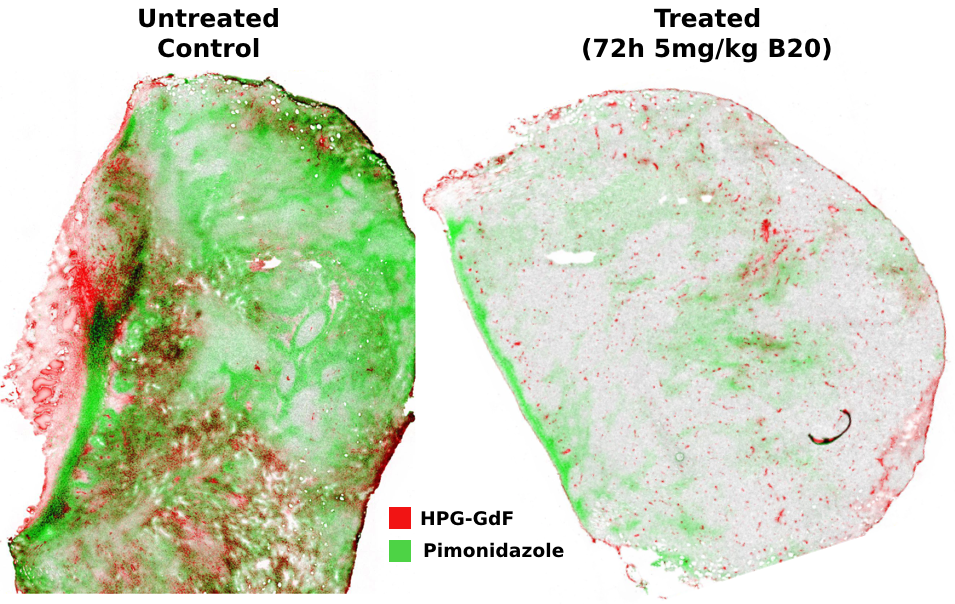
\includegraphics[width=\textwidth]{hpg/hpg-B20-images/histo_hpgPimo.png} 
  \captionsetup{width=\linewidth}
  \caption{Histological sections of a control (left) and treated tumour (right) are shown to illustrate the dramatic decreases both in pimonidazole staining and in accumulation of \acs{HPG-GdF} in the treatment group.}
  \label{hpgB20:histohpgpimo}
\end{figure}

Quantitative analysis of the immunohistolgoical stains in the images was conducted to assess whether these observations existed at the group level. 
A Mann-WhitneyU test indicated that the median pimonidazole staining intensity was greater for the control group ($I_{pimo}$ = 21.7) than the treated group ($I_{pimo}$ = 17.2), $U = 47$, $p = 5\times10^{-5}$.
Median \acs{HPG-GdF} staining intensity is also reduced for the treated tumours ($I_{hpg} = 12.7$) compared to the controls ($I_{hpg} =11.0$), Mann-Whitney$U=52$, $p = 8\times10^{-6}$.
Data for individual tumours as well as the group differences are shown in figure~\ref{hpgB20:accumulation}.

\begin{figure}[htbp] % figure placement: here, top, bottom, or page
  \centering
  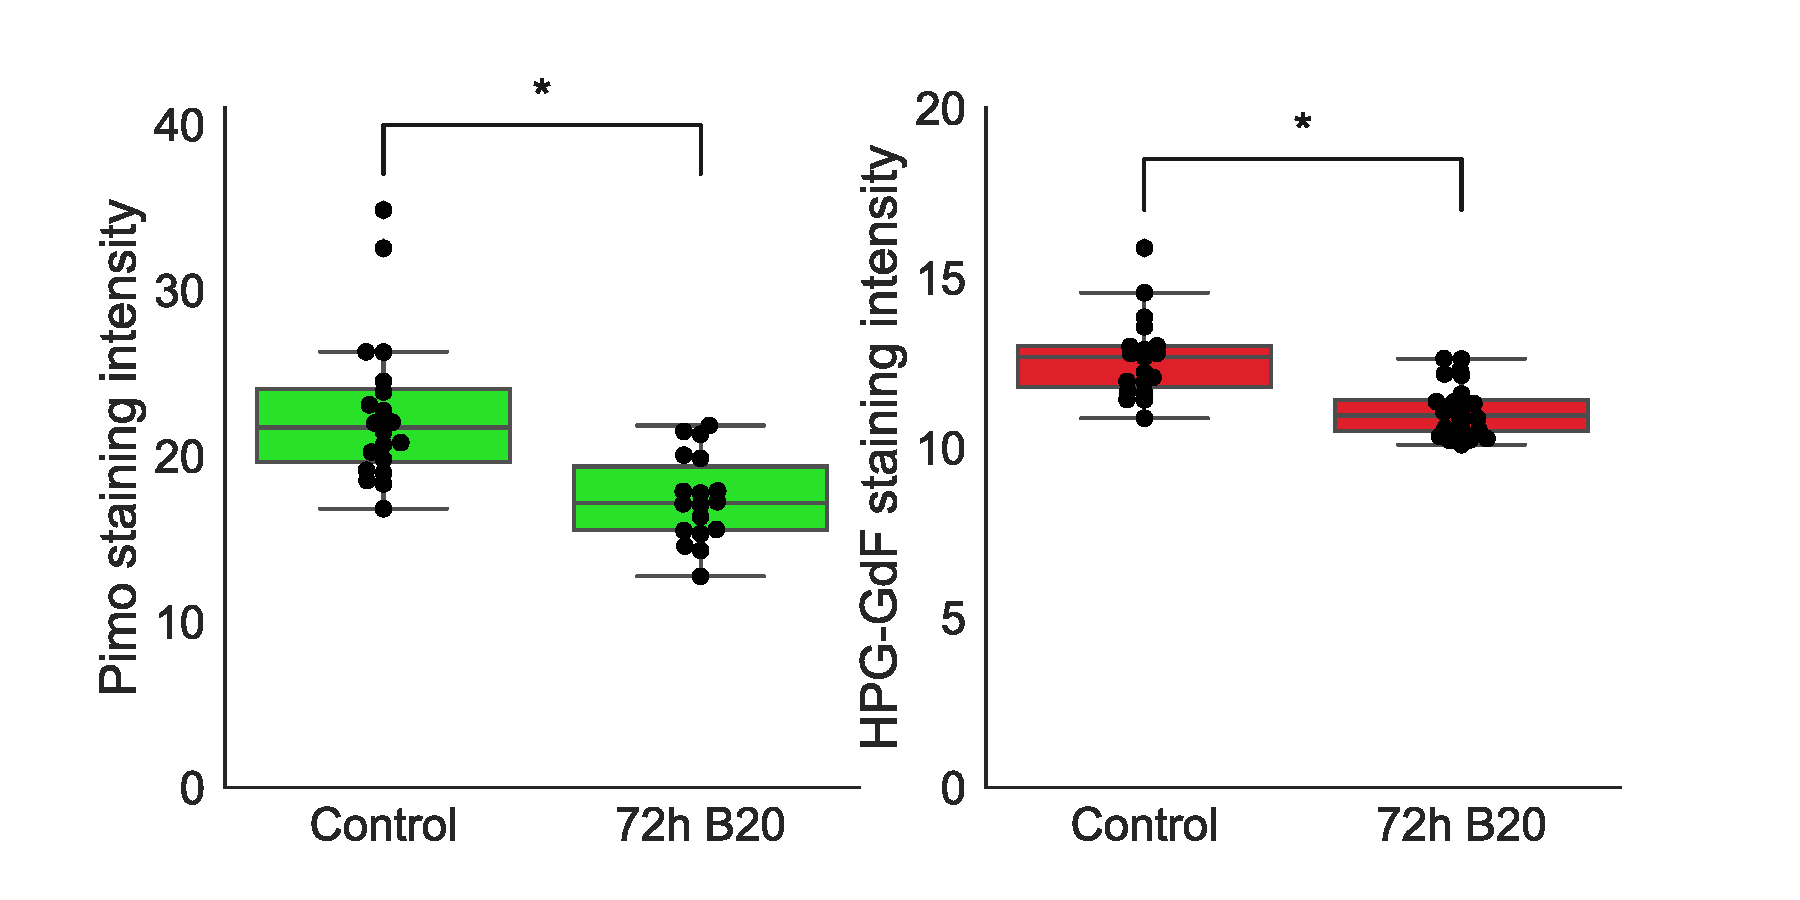
\includegraphics[width=\textwidth]{hpg/hpg-B20-images/hpg_pimoHPG-GdF.pdf}
  %\captionsetup{width=\linewidth}
  \caption{Median pimonidazole staining is markedly reduced for the B20-treated group ($I_{pimo} = 17.2$) compared to the controls ($I_{pimo} = 21.7$).
  Median \acs{HPG-GdF} staining intensity is also reduced for the treated tumours ($I_{hpg} = 12.7$) compared to the controls ($I_{hpg} =11.0$).
  P-values from the Mann-WhitneyU test were $p = 5\times10^{-5}$ (pimo, left) and $p = 8\times10^{-6}$ (\acs{HPG-GdF} fluorescence, right).}
  \label{hpgB20:accumulation}
\end{figure}

\begin{figure}[htbp] % figure placement: here, top, bottom, or page
  \centering
  \includegraphics[width=\textwidth]{hpg/hpg-B20-images/hpg_allHisto.pdf} 
  \captionsetup{width=\linewidth}
  \caption{all histo pimo}
  \label{hpg:allHisto}
\end{figure}

\subsection{Blood vessel permeability (\acs{aPS}) and HPG-GdF accumulation (fluorescence intensity) decreases in tumours treated with B20}

Apparent permeability-surface area product (\acs{aPS}) is a parameter that captures vessel leakiness with \acs{DCE-MRI} using the large molecular weight contrast agent~\acs{HPG-GdF}.
Figure~\ref{hpgB20:mriparams} shows the group differences and the median value of the B20-treated group (aPS$_{Md}$ = $1\times10^{-4}$) was significantly lower than the control group (aPS$_{Md}$ = $6.5\times10^{-5}$); Mann-Whitney $U = 3$, $p = 0.01$.

Histological staining of \acs{HPG-GdF} fluorescence matched relatively well with areas of high \acs{aPS} values as shown in figure~\ref{hpg:aPShistoEC}, however there are also areas where aPS is moderate or high but \acs{HPG-GdF} fluorescence is not present in high concentrations. 
Group differences in \acs{HPG-GdF} accumulation were also present histologically as \acs{HPG-GdF} fluorescence intensity was markedly decreased in the B20-treated tumours ($I_{hpg} = 12.7$) compared to the controls ($I_{hpg} = 11.0$); a Mann-WhitneyU test indicated the difference was significant $U = 52$, $p = 9\times10^{-6}$.
Aggregate voxel distributions of \acs{aPS} values in Figure~\ref{hpgB20:accumulation} also shows a clear reduction in \acs{aPS} in the treatment group.Figure~\ref{hpg:aPShistoEC} shows the \acs{aPS} parametric maps from \acs{DCE-MRI} alongisde approximate slice matched histology sections from the same tumours.
Patterns observed in the quantitative analysis of the data are also evident in MRI and histology images: following treatment with B20, there is a marked reduction in blood vessel permeability measured by \acs{aPS} and a reduction in \acs{HPG-GdF} accumulation histologically measured by native fluorescence of the contrast agent.

\begin{figure}[htbp] % figure placement: here, top, bottom, or page
  \centering
  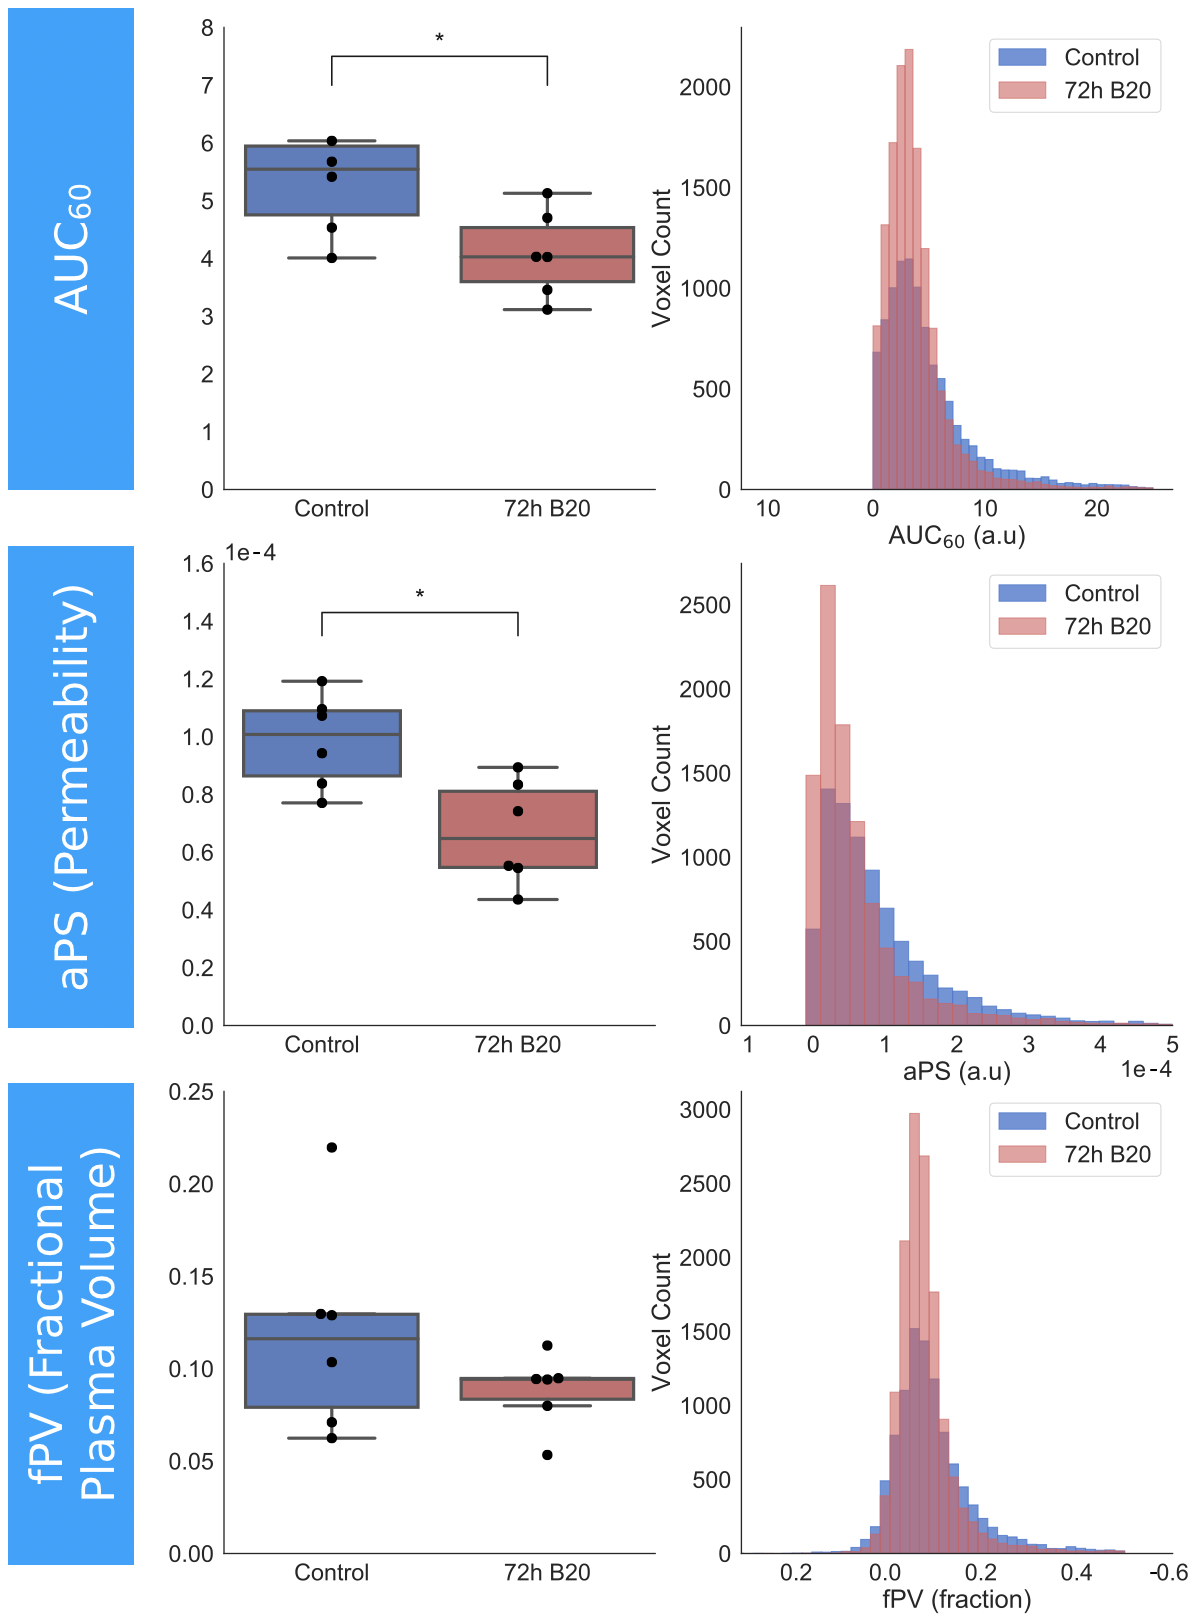
\includegraphics[width=0.8\textwidth]{hpg/hpg-B20-images/hpg_mriparams.png} 
  %\captionsetup{width=\linewidth}
  \caption{Summary of group differences for all three \acs{DCE-MRI} parameters: \acs{AUC}$_{60}$, \acs{aPS}, and \acs{fPV}. 
  There is a statistically significant reduction in \acs{AUC}$_{60}$ and \acs{aPS} for the treated tumours, but no difference measured for \acs{fPV}.
  P-values from the Mann-WhitneyU statistical test for the comparisons were $p=0.03$ (\acs{AUC}$_{60}$), $p=0.01$ (\acs{aPS}), and $p=0.15$ (\acs{fPV}).}
  \label{hpgB20:mriparams}
\end{figure}

\subsection{\acs{HPG-GdF} enhancement curves and \acs{AUC}$_{60}$ are altered after treatment, but \acs{fPV} does not change}

Group \acs{HPG-GdF} enhancement curves are shown in Figure~\ref{hpg:aPShistoEC} and match the results obtained from a quantitative analysis of the parameteric maps: treated tumours have a relatively flat profile and plateau whereas the control tumours show a steady increase of enhancement arising from the leakage of \acs{HPG-GdF}.
\acs{AUC}$_{60}$ is a parameter that captures the relative enhancement of voxels within the first 60 seconds after injection.
The control tumours had a median \acs{AUC}$_{60-Md} = 5.5$ and treated tumours had a median \acs{AUC}$_{60-Md} = 4.0$ and the reduction was statistically significant (Mann-Whitney $U = 6, p = 0.03$).
The \acs{fPV} values for the control (fPV$_{Md} = 0.12$) and treated tumours (fPV$_{Md} = 0.09$) were not significantly different (Mann-Whitney $U = 3, p = 0.15$).

\begin{figure}[htbp] % figure placement: here, top, bottom, or page
  \centering
  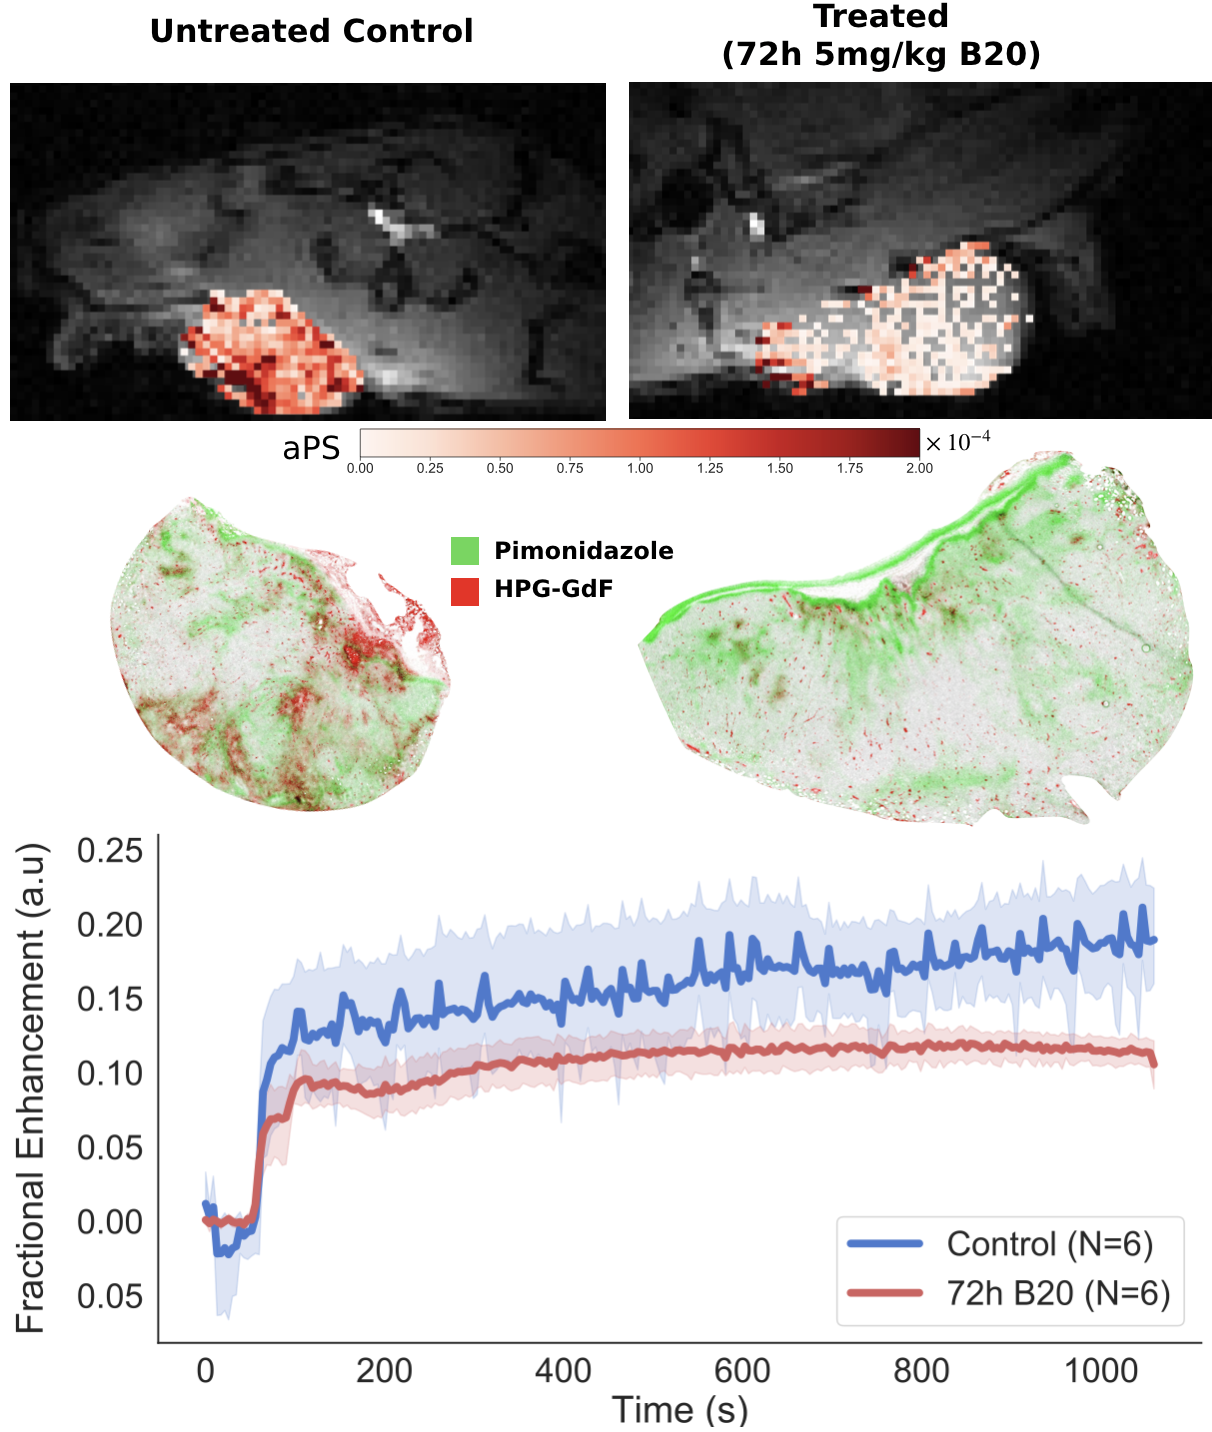
\includegraphics[width=0.8\textwidth]{hpg/hpg-B20-images/hpg_aPShisto_ec.png} 
  \captionsetup{width=\linewidth}
  \caption{Histological stains of \acs{HPG-GdF} shown alongside approximate slice matched \acs{DCE-MRI} parameter map of \acs{aPS} and the group-averaged contrast enhancement curves of control and treated tumours. There is an overall reduction in \acs{aPS} for the treated tumours. The mean contrast enhancement curves (group means in dark blue and red lines; shaded region is the 95\% confidence interval determined by bootstrapping) also show that the treated tumours have a higher enhancement slope after contrast agent injection.}
  \label{hpg:aPShistoEC}
\end{figure}

\section{Discussion}

In this study we have demonstrated that vessel permeability can be assessed using the apparent permeability-surface area product, \acs{aPS}.
This is consistent with similar reports of extracting permeability parameters with \acs{DCE-MRI} using albumin-based macromolecular contrast agents~\cite{DaldrupLink:2004gy,Turetschek:2001wu}, dendrimer-based contrast agents~\cite{deLussanet:2005cb} and others~\cite{Turetschek:2004bw}.
Typically, contrast agents used in \acs{DCE-MRI} are less than 1 kDa in molecular weight and freely extravasate from vessels and enhance surrounding tissues.
These low molecular weight agents are essential for many applications including cancer detection,  evaluating vascular characteristics, and measuring tumour microenvironment changes longitudinally~\cite{Padhani:2002cj}.
However, there is a strong coupling of blood flow and vessel permeability in standard \acs{DCE-MRI} models parameter interpretation varies based on the tumour microenvironment~\cite{Gerstner:2008ba}.
For instance, in regions of high permeability, the movement of the contrast agent is limited by blood flow so \acs{K$^{trans}$} primarily measures blood flow.
When applied in regimes of low permeability, the small molecular weight contrast agent cannot extravasate from vessels so \acs{K$^{trans}$} primarily measures vessel permeability~\cite{Tofts:1999we}.
Contrast agent size affects measures of vascular permeability and low molecular weight agents result in underestimations of vessel permeability ~\cite{deLussanet:2005cb}.
For applications where distinguishing between blood flow and vessel permeability is important, low molecular weight agents cannot be used.

The principal advantage of high molecular weight contrast agents is their intravascular nature so blood flow is removed as a contributing factor of the measurement.
There is also an inverse relationship between size of the contrast agent and MR signal enhancement because larger molecules diffuse slower and extravasate less.
The reduction in signal enhancement is partially compensated for by the increased relaxivity of the larger agent arising from more Gd-chelates attached to the molecule and a lower tumbling rate~\cite{Barrett:2006jx}.
We have previously shown that the relaxivity of ~\acs{HPG-GdF} is 300 times larger than standard \acs{DCE-MRI} contrast agents but the agent extravasates only a few micrometers from nearby vessels~\cite{Baker:2015coa}, leading to an overall reduction in signal enhancement.
In summary, the larger the contrast agent, the less signal enhancement there is in the MR images and \acs{HPG-GdF} has a molecular weight of 583 kDa.
This is considerably larger than common biocompatible high molecular weight agents that range from 20-92 kDa~\cite{Barrett:2006jx} and to our knowledge, \acs{HPG-GdF} is the largest agent with which a permeability measure has been obtained.

This study provides another application for the high molecular weight agent \acs{HPG-GdF} in exploring the tumour microenvironment and the effects of vascular normalization.
\acs{AUC}$_{60}$ of the signal intensity represents presence of HPG in the blood 60s after injection was also significantly lower in the treated mice which indicates the antiangiogenic treatment altered the tumour vasculature.
There is considerably less variability in the enhancement curves of the treated tumours as shown in Figure~\ref{hpg:aPShistoEC},providing strong evidence for B20 normalizing the vasculature.
The vascular normalization hypothesis suggests that after treatment with an antiangiogenic therapy, the overall vessel permeability and the number of vessels will decrease.
Our study has provided evidence for a decrease in vessel permeability through \acs{aPS} and a decrease in accumulation of \acs{HPG-GdF} through \acs{AUC}$_{60}$ (See figure~\ref{hpgB20:mriparams}).
Additionally, we also showed a dramatic reduction in hypoxia (measured by pimonidazole staining) in the treated group. 
Existing MRI techniques do not permit measurement of oxygenation \emph{in vivo} despite an unmet clinical need~\cite{Horsman:2012kw}.

\todo{Transition needs some work here} While the SCCVII cell line is a murine model, it is ideal for validating non-invasive MRI as it has almost no necrosis present due to its vascular architecture.
Necrosis is a potential confounding factor in macromolecular contrast agent imaging studies as large areas of necrosis and empty space result in pooling of the agent in non-viable areas.
Consequently in SCCVII tumours, any fluorescence present on cryosections has extravasated from nearby vessels and can be quantified as shown in figure~\ref{hpgB20:accumulation}.
Figure~\ref{hpg:allHisto} shows low inter-tumour slice variability in average staining intensity of \acs{HPG-GdF} fluorescence, but considerable heterogeneity exists between tumours and not all tumours responded consistently.
On aggregate it is evident that the treated tumours have significantly less HPG accumulation.
Figure~\ref{hpg:allHisto} also shows regions stained with both \acs{HPG-GdF} and pimonidazole.
There is no clear explanation for why a macromolecule such as \acs{HPG-GdF} accumulates in a region where oxygen is regionally distributed in such low concentrations.
One possible explanation is that in longer imaging sessions tumors exhibit varying oxygenation patterns and since pimonidazole and \acs{HPG-GdF} were administered over two hours apart, the tumour microenvironment had changed. 
Periods of oxygen-starvation and re-oxygenation cycling in tumors has been termed cycling hypoxia and can arise for intermittent periods based on temporary vessel occlusions, or may be permanent, chronic changes in hypoxia~\cite{Dewhirst:2009de,Michiels:2016hv}.
However as has been recently demonstrated, it is not as simple as classifying tumours in a binary fashion~\cite{Bayer:2011js}.
To enable a more thorough exploration of this phenomenon, more sophisticated methods are needed including a non-invasive method of assessing oxygenation status ~\emph{in vivo} validated with multiple stains of hypoxia such as pimonidazole and EF5 administered sequentially with a delay to capture any changes that occur during the delay time.
Additionally, slice-matched histology sections and MR images were beyond the scope of this study and this would be needed to explore patterns of \acs{HPG-GdF} staining and regions of high \acs{aPS} or \acs{fPV}.

An important difference in this study compared to our initial experiments with \acs{HPG-GdF}~\cite{Baker:2015coa} is that here we analyzed only the signal intensity enhancement rather than relying on an arterial input function to compute a contrast agent concentration.
Largely due to constraints in available signal enhancement due to the high molecular weight contrast agent, sufficient signal was not present in all areas of the tumour fir pharmacokinetic modeling or computation of contrast agent concentration.
Though this simplification is not ideal as it assumes signal intensity changes linearly with contrast agent concentration, it is valid when contrast agent concentrations are low~\cite{Heilmann:2006bm} and relative group differences are being measured (rather than absolute changes in individual tumours).
This and other challenges associated with a lack of standardization in analysis methods to use high molecular weight contrast agents poses a significant challenge for its use in the clinic as a tool to assess cancer therapies. 
Nevertheless, validation with histological images is a positive sign that the measurements of \acs{aPS} and \acs{fPV} reflect characteristics of the tumour microenvironment.

\section{Conclusion}

We have shown that \acs{aPS} and \acs{AUC}$_{60}$ decreases after administration of B20.
Lower accumulation of \acs{HPG-GdF} following treatment was confirmed by histology via direct \acs{HPG-GdF} fluorescence imaging.
Blood vessels of treated tumours appear to be less permeable as a result of the anti-angiogenic drug.
Our results indicate that \acs{HPG-GdF} has potential applications is assessing effects of antiangiogenic agents on blood vessel permeability and function.
Future work will include a panel of tumours with radically different tumour microenvironments to evaluate its utility in more clinically relevant tumour models.
While it is unclear that macromolecular contrast agents will become standard clinically, they are a very useful tool to improve our understanding of the tumour microenvironment and to develop novel drugs for cancer.
\endinput